\pagebreak\section{Measurement of voltages (Below 5V and above)}
\subsection{Experiment URL}
    Use this \href{https://www.tinkercad.com/things/awpboVDdbxj?sharecode=uw7s84LgESyuaN5hnURGDUiU3aelHYsxpXATCcO_EfU}{link} to get the \textbf{Tinkercad} simulation of this experiment.
\subsection{Objectives}
We are going to make a simple digital voltmeter using the Arduino Uno R3, which can safely measure input dc voltages in 0 to 30V range. The Arduino board can be powered from a standard 9V battery pack or you can just use your desktop's USB port, as usual.

As you may well know, Arduino’s analog inputs can be used to measure DC voltage between 0 and 5V (when using the standard 5V analog reference voltage) and this range can be increased by using two resistors to create a voltage divider. The voltage divider decreases the voltage being measured to within the range of the Arduino analog inputs. Code in the Arduino sketch is then used to compute the actual voltage being measured.

\subsection{Necessary Components}
We will need the following components −
\begin{itemize}
\item 1 x Arduino Uno R3
\item 1 x Breadboard
\item 1 x 30V Power Supply
\item 1 x 1k$\Omega$ Resistor
\item 1 x 5k$\Omega$ Resistor
\item 1 x 16x2 LCD screen
\item 1 x USB A-B cable
\item Jumper Wires
\end{itemize}


\subsection{Circuit Diagram}
            \begin{center}
            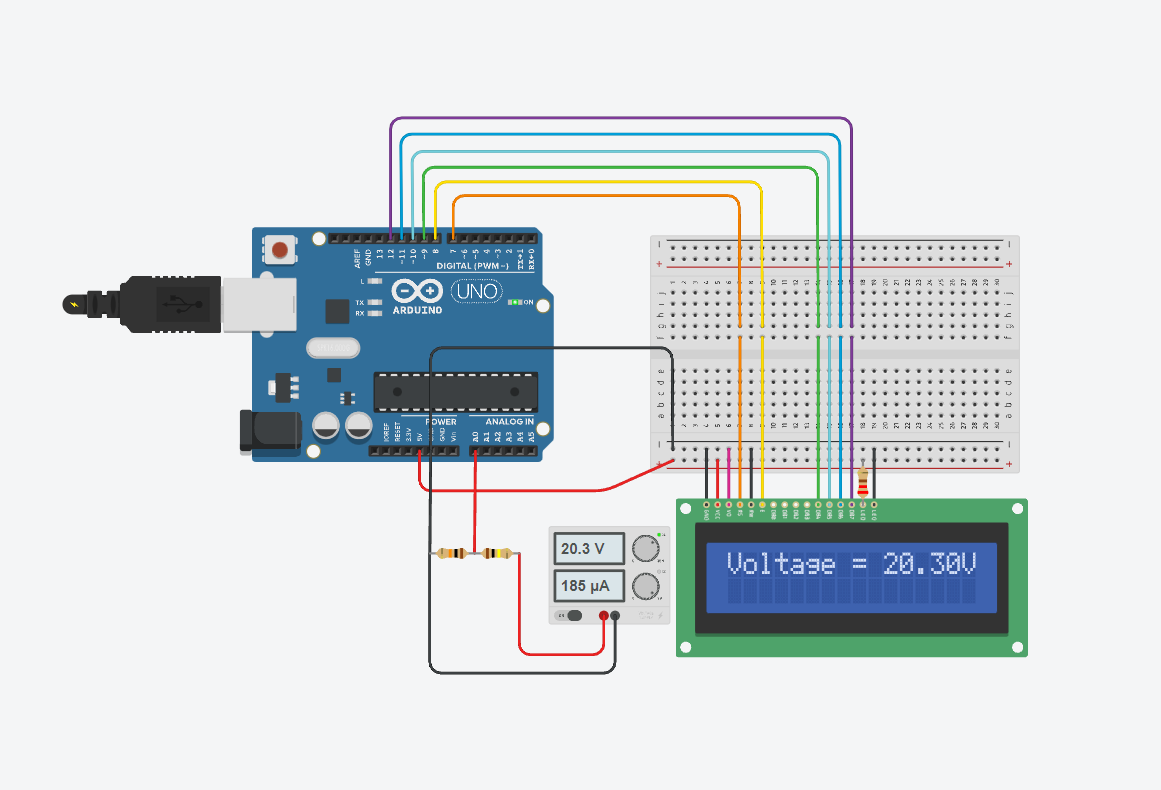
\includegraphics[width =0.85\textwidth]{images/measure_analog_voltage.png}
            \end{center}


\subsection{Formula for calculating voltage:}

\begin{equation}
    V_0 = (Val * 5.0) / 1023.00
\end{equation}
Here in these formula Val is the value that is read by Arduino as analog input, which is further multiplied by the voltage that is been supplied by Arduino and thus to get the Vout it is divided by the cycle of time that is covered after every bit to get the value.
\begin{equation}
    V_{in} = {V_{0}}~/~\frac{R2}{(R1+R2)}
\end{equation}
Using this formula we can convert the high voltages into the voltage range of Arduino (0 - 5V) using the voltage divider and measure any voltage using suitable resistor combinations. 

NOTE: Here there is no restriction on using the specified amount of resistors, one can vary it according to the availability of the resistors.


\pagebreak\subsection{Arduino Code}
    \begin{lstlisting}[style = Arduino]
/*Analog voltage measurement using Arduino*/

#include <LiquidCrystal.h>

//initialize the library by associating needed LCD interface pin
const int rs = 7, en = 8, d4 = 9, d5 = 10, d6 = 11, d7 = 12;

LiquidCrystal lcd(rs, en, d4, d5, d6, d7);

int analogIn = A0;
float v0 = 0.0;
float vin = 0.0;
float R1 = 5000.0; // resistance of R1 (5K) 
float R2 = 1000.0; // resistance of R2 (1K) 
int value;
void setup()
	{
   pinMode(analogIn, INPUT);
   lcd.begin(16, 2);
   lcd.setCursor(4,0);
   lcd.print("Voltmeter");
   delay(1000);
  	}

void loop()
	{
  value = analogRead(analogIn);  //read the value at analog input pin
  v0 = (value * 5.0) / 1023.0; // voltage value as read by A0
  vin = v0 / (R2/(R1+R2)); // voltage reverted back to original

  lcd.clear();
  lcd.setCursor(0, 0);
  lcd.print("Voltage = ");
  lcd.print(vin);
  lcd.print("V");
  delay(100);
}
    \end{lstlisting}